\documentclass[conference]{IEEEtran}
\IEEEoverridecommandlockouts
\usepackage{cite}
\usepackage{amsmath,amssymb,amsfonts}
\usepackage{graphicx}
\usepackage{booktabs}
\usepackage{multirow}
\usepackage{xcolor}
\usepackage{tikz}
\usetikzlibrary{arrows.meta,positioning,fit}
\usepackage[hidelinks]{hyperref}

\newcommand{\up}{\mathcal{U}}
\newcommand{\dn}{\mathcal{D}}

\begin{document}

\title{JA-NPR: JPEG-Aware Neighboring Pixel Relationships\\for Compression-Robust Deepfake Detection}

\author{
\IEEEauthorblockN{Pranav Vinod and Shrija Tewari}
\IEEEauthorblockA{Netaji Subhas University of Technology\\
New Delhi, India}
}

\maketitle

\begin{abstract}
NPR looks for CNN up-sampling by subtracting, inside every $2{\times}2$ cell, the top-left pixel from the other three. The released 1.44M checkpoint ranks AttGAN faces well on PNG and still does so at JPEG quality 95 if chroma is stored at full resolution. The same files saved 4:2:0 invert the ranking. After decoding, the colour differences inside a cell are the interpolator's, not the generator's.
JA-NPR leaves that cell operator in place. Luma is still residualized at full resolution. Chroma is average-pooled to $2{\times}2$ and residualized there, on the decoded pixels. Each batch-norm keeps a clean buffer and a JPEG buffer, and a zero-initialized FiLM layer reads a four-number header summary. The extra cost is 50{,}560 parameters. Against an NPR fine-tune that sees the same crops, the same face-disjoint splits, and a pass rule written down before the runs, the three-seed AttGAN mean at Q95 4:2:0 moves from 0.799 to 0.922, and JA-NPR is ahead at every JPEG quality in the table. A constant header vector matches that AttGAN number, so the table entries themselves are not what the training generator is using. A higher learning rate on the old batch-norm scale and shift does not match it either. On seven generators held out of training, the normalization transfers more often than the header values do. The header helps STGAN on both seeds we ran and hurts InfoMaxGAN and S3GAN. Several earlier variants, including a quantization-bin projection and a compression-adversarial head, did not beat the fine-tune.
\end{abstract}

\begin{IEEEkeywords}
Deepfake detection, JPEG compression, neighboring pixel relationships, chroma subsampling, quantization table, conditional normalization
\end{IEEEkeywords}

% =====================================================================================
\section{Introduction}
Most detector papers train and test on PNG. The files people actually pass around are JPEG, and high-frequency cues are known to fall apart once blur or compression is applied~\cite{wang2020cnndetection,frank2020frequency,le2023qad}.

NPR~\cite{tan2024npr} is small enough that we could change it and still know what we had changed. CNN up-samplers, nearest-neighbour and transposed convolution, leave the four pixels of a $2{\times}2$ cell too alike. NPR subtracts the top-left pixel of the cell from the others and feeds the residual to a truncated ResNet~\cite{he2016resnet}. Tan et al.\ report that this cue transfers across generators. We take that claim as the reason to start from their checkpoint, not as something we re-tested on clean data.

On AttGAN the released weights are fine on PNG (AUC 0.956). Save the same faces at quality 95 with 4:4:4 chroma and the AUC is still 0.876. Save them 4:2:0 and it falls to 0.233, which means fakes are ranked as more real than reals. Quality 95 is not a heavy quantizer. The drop lines up with chroma subsampling. Quantization is not innocent either: at Q75 the released model is inverted even with 4:4:4 (AUC 0.365).

A 4:2:0 file stores one Cb and one Cr per $2{\times}2$ cell. After a smooth upsample, the other three colour samples in the cell are filled in by the decoder. NPR then treats that fill as if the generator had written it. The luma residual is also changed, by an amount that depends on the quantization table in the header. Those two facts are the whole design.

We keep NPR's cell and make two changes. Chroma-aligned NPR (CA-NPR) residualizes luma at full resolution and chroma after a $2{\times}2$ average pool, which is the grid a 4:2:0 file stores. The first convolution can be rewritten so that, with full-resolution chroma, the network starts at the released weights. The pooled path is the part that actually differs at initialization, and it adds no parameters. QT-Norm gives every batch-norm two running-stat buffers, one for files with a quantization table and one without, and a FiLM map~\cite{perez2018film} from a four-number header vector. The FiLM weights start at zero. The new parameters total 50{,}560.

The baseline is not the released checkpoint. It is that checkpoint fine-tuned on the same clean-plus-JPEG crops. AttGAN is split by source face, intervals are paired cluster bootstraps, and the pass rule was in the code before these runs. Three seeds redraw the split. We also train with SNGAN in the mix and test generators that were never in that mix. The header is checked so that it cannot stand in for the label. Variants that lost are in the paper, not only the one we kept.

Three controls are there to stop a loose reading of the gain. One feeds FiLM a constant vector, same parameter count, no header values. One raises the learning rate on the batch-norm scale and shift that were already in NPR. One puts QT-Norm on the original RGB residual and leaves chroma pooling out. On AttGAN the constant vector matches JA-NPR and the learning-rate control does not. The chroma pool, measured against RGB QT-Norm, is a small and condition-dependent difference.

% =====================================================================================
\section{Related Work}
Up-sampling leaves traces that several detectors read directly: spectral peaks~\cite{frank2020frequency}, gradients~\cite{tan2023lgrad}, and the local pixel dependence NPR uses~\cite{tan2024npr}. Wang et al.~\cite{wang2020cnndetection} showed that if blur and JPEG are in the training augmentation, a CNN detector survives them better at test time. That result tells you to train on compressed images. It does not say which part of the JPEG pipeline removed the cue.

QAD~\cite{le2023qad} pulls the features of a low-quality view and a high-quality view toward each other. ODDN~\cite{tao2025oddn} and PLADA~\cite{li2025plada} train on images that have been through social-network compression, with paired or unpaired views and an adversarial term that tries to hide the compression from a second head. Those models sit on large backbones. We stay on NPR's trunk and add about 0.05M parameters.

Restoration networks already condition on a quality factor or on the quantization table itself~\cite{jiang2021fbcnn,ehrlich2020qgac}. Domain-specific batch-norm stores a separate mean and variance per domain~\cite{chang2019dsbn}. FiLM applies a scale and a shift computed from a side vector~\cite{perez2018film}. QT-Norm is those last two ideas, with the JPEG header as the side vector, inside the NPR batch-norm layers. We have not found a previous NPR detector that reads the table this way. If one exists, our comparison is still against a matched fine-tune of the released NPR weights, not against that other system.

The practical difference from QAD, ODDN and PLADA is the question being asked. Those methods train a large network to ignore compression. We ask why this particular residual fails when chroma is subsampled, then change the resolution at which chroma enters the residual and the statistics the batch-norm uses on a JPEG file. The controls later in the paper put most of the AttGAN gain on the normalization, not on the chroma pool. We do not claim a detector that is robust on every generator, and we do not run the large compression-robust models as baselines.

% =====================================================================================
\section{Why NPR Fails Under JPEG}
\label{sec:why}
JPEG~\cite{wallace1992jpeg} converts RGB to YCbCr, then, in the usual 4:2:0 setting, keeps chroma at half the luma resolution. Each $2{\times}2$ cell is left with one Cb value and one Cr value. The $8{\times}8$ DCT coefficients are divided by the quantization table, and that table is stored in the header. On the way back out, chroma is interpolated up to the luma grid.

NPR's residual uses two operators. $\dn$ keeps the top-left pixel of every $2{\times}2$ cell and $\up$ repeats it across the cell:
\begin{equation}
R(x) = x - \up(\dn(x)).
\end{equation}
On a 4:2:0 decode, the chroma part of $R$ is whatever the interpolator put inside the cell (Fig.~\ref{fig:chroma}). It is a function of neighbouring stored samples. It is not a function of a within-cell colour pattern the generator wrote, because that pattern was never stored.

A probe with no extra training makes the same point. We take NPR after the earlier JPEG fine-tune (protocol P1, Section~\ref{sec:fail}) and, on AttGAN at Q95 4:2:0, replace decoded chroma by a single value in each $2{\times}2$ cell. AUC goes from 0.829 up to 0.864. The same replacement on PNG goes from 0.999 down to 0.863. When the colour detail is real, the detector uses it. When the decoder invented it, throwing it away helps.

Fig.~\ref{fig:residuals} is one AttGAN fake, cropped to $48{\times}48$. The RGB residual, which is mostly luma, still looks like the face after Q95 4:2:0. The Cb residual does not. 4:4:4 at the same quality keeps more of the in-cell colour structure than 4:2:0 does.

\begin{figure}[t]
\centering
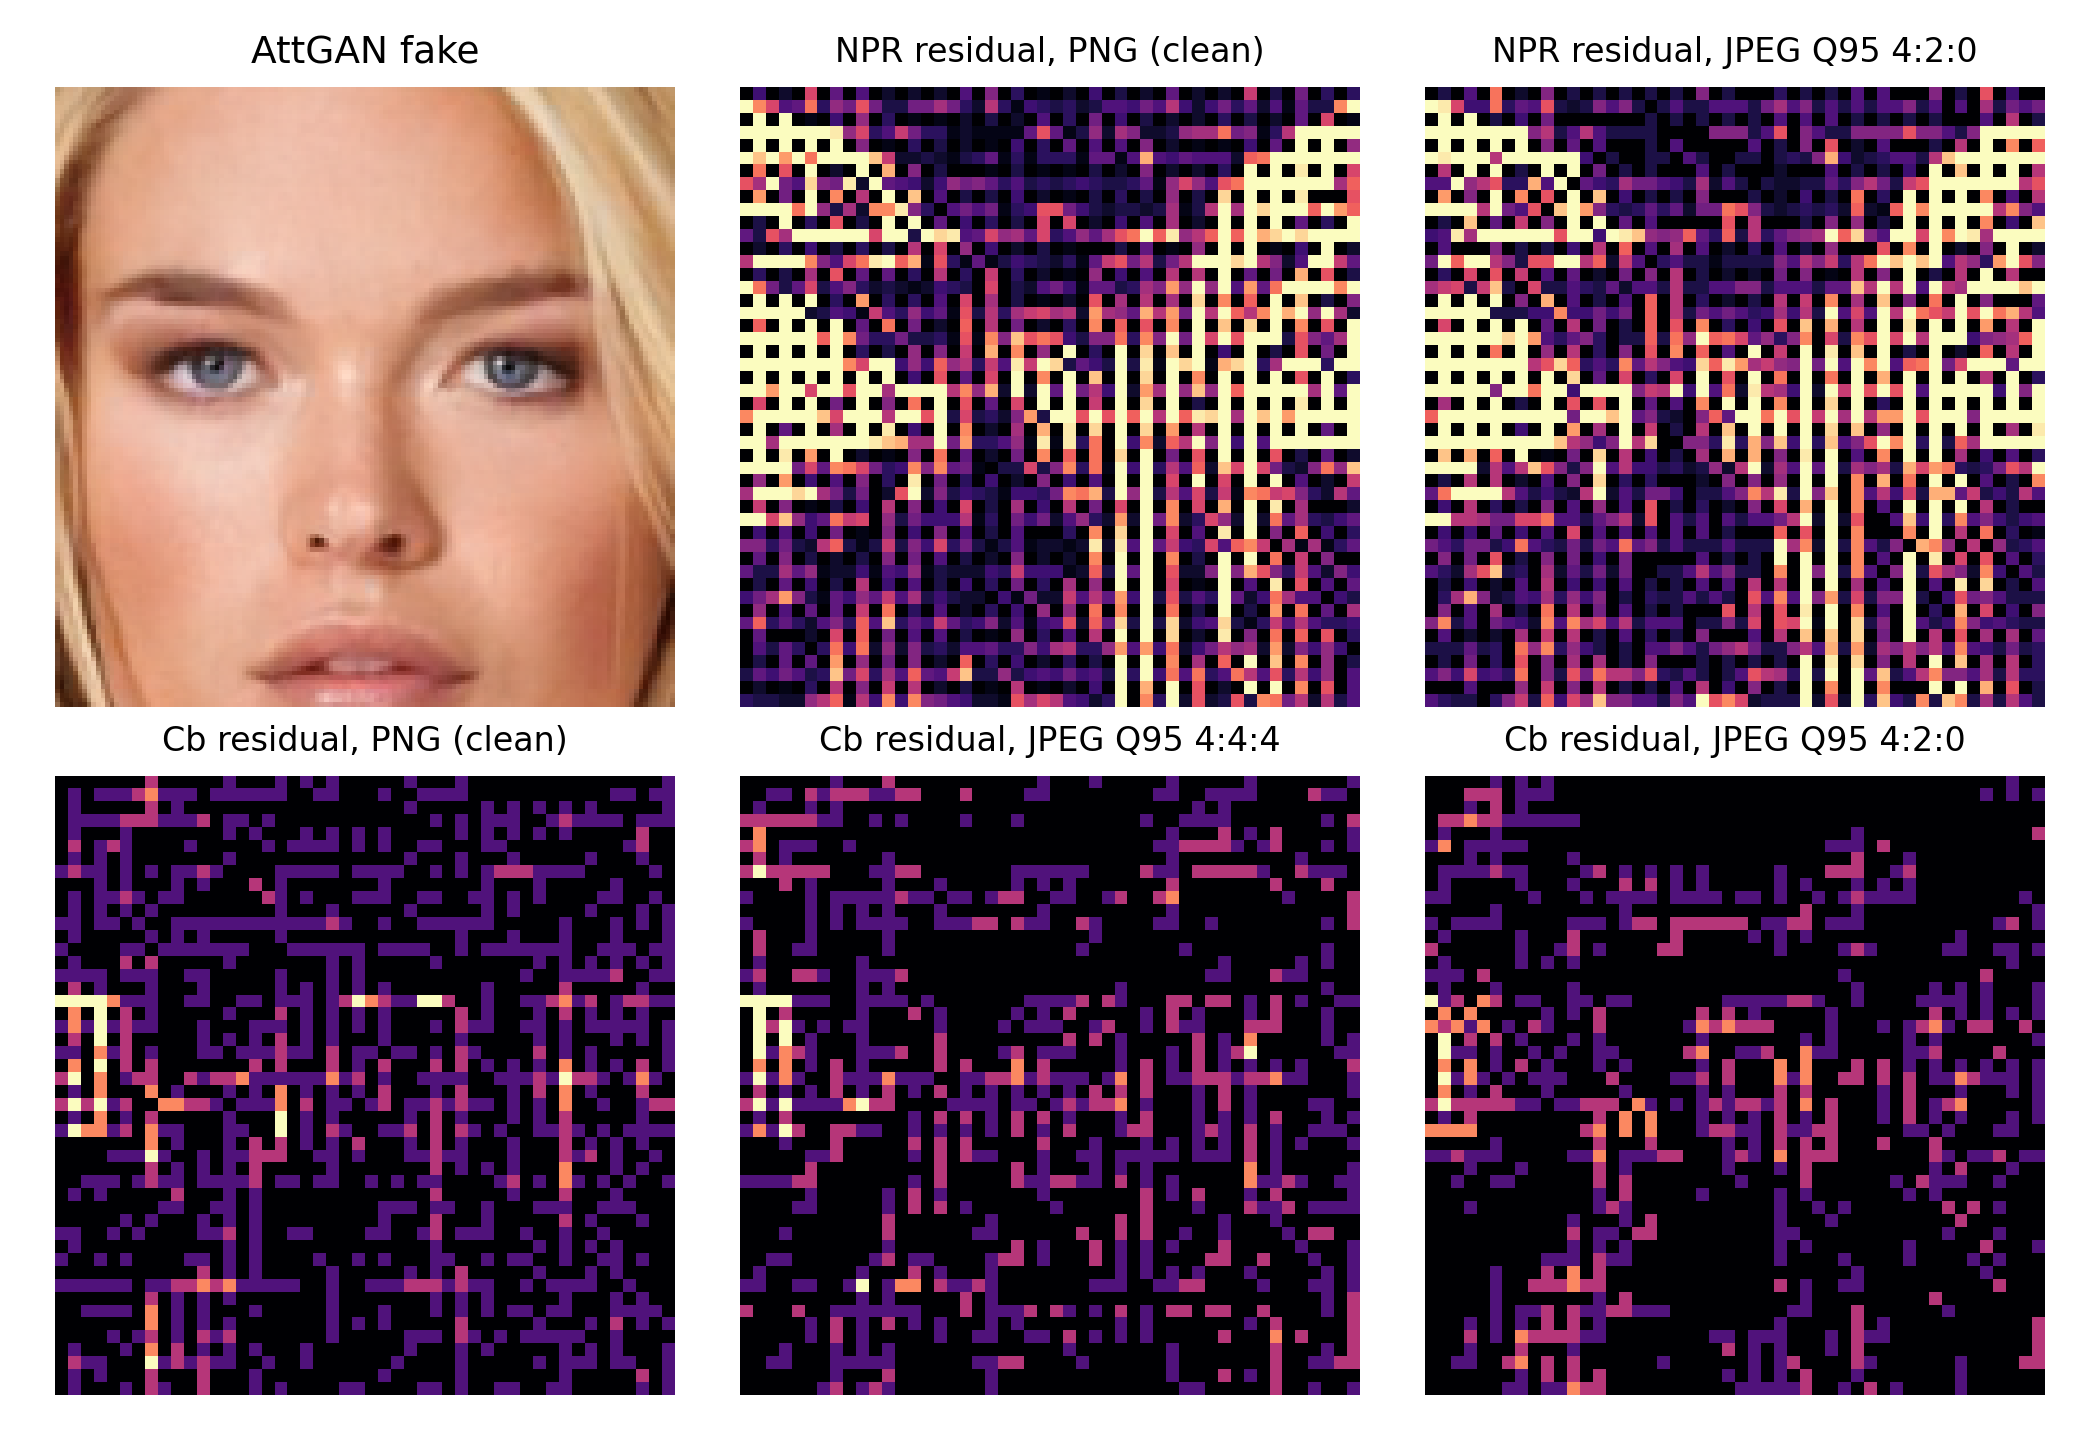
\includegraphics[width=\columnwidth]{figures/fig_residuals.png}
\caption{NPR residuals of an AttGAN fake ($48{\times}48$ crop; brighter means larger
$|x-\mathcal{U}(\mathcal{D}(x))|$). Top: the face, and the NPR residual (mean over RGB) for the
PNG and for JPEG Q95 4:2:0. Bottom: the residual of the Cb colour channel for the PNG, JPEG Q95
4:4:4 and JPEG Q95 4:2:0. Under 4:2:0, much of the in-cell colour structure is lost.}
\label{fig:residuals}
\end{figure}

\begin{figure}[t]
\centering
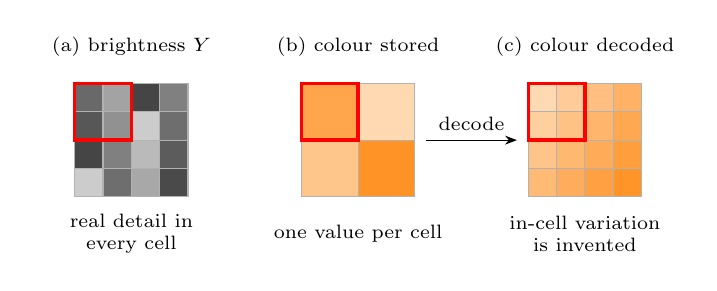
\begin{tikzpicture}[font=\scriptsize, x=0.36cm, y=0.36cm]
\foreach \i in {0,...,3}{\foreach \j in {0,...,3}{
  \pgfmathsetmacro{\g}{20+mod(\i*37+\j*53,60)}
  \fill[black!\g] (\i,\j) rectangle ++(1,1);}}
\draw[step=1,gray!60] (0,0) grid (4,4); \draw[very thick,red] (0,2) rectangle (2,4);
\fill[orange!70] (8,2) rectangle (10,4); \fill[orange!30] (10,2) rectangle (12,4);
\fill[orange!45] (8,0) rectangle (10,2); \fill[orange!85] (10,0) rectangle (12,2);
\draw[step=2,gray!60] (8,0) grid (12,4); \draw[very thick,red] (8,2) rectangle (10,4);
\foreach \i in {0,...,3}{\foreach \j in {0,...,3}{
  \pgfmathsetmacro{\c}{30+10*\i+8*(3-\j)}
  \fill[orange!\c] (16+\i,\j) rectangle ++(1,1);}}
\draw[step=1,gray!60] (16,0) grid (20,4); \draw[very thick,red] (16,2) rectangle (18,4);
\draw[-{Stealth[length=1.5mm]}] (12.4,2) -- (15.6,2) node[midway,above]{decode};
\node[align=center,text width=2.3cm] at (2,5.3) {(a) brightness $Y$};
\node[align=center,text width=2.3cm] at (10,5.3) {(b) colour stored};
\node[align=center,text width=2.3cm] at (18,5.3) {(c) colour decoded};
\node[align=center,text width=2.4cm] at (2,-1.3) {real detail in every cell};
\node[align=center,text width=2.4cm] at (10,-1.3) {one value per cell};
\node[align=center,text width=2.4cm] at (18,-1.3) {in-cell variation is invented};
\end{tikzpicture}
\caption{Why 4:2:0 JPEG misleads NPR. The red square is one NPR $2{\times}2$ cell. Brightness keeps
real detail inside the cell, but colour is stored once per cell. The variation that NPR measures
inside the cell after decoding is created by the decoder's interpolation, not by the generator.}
\label{fig:chroma}
\end{figure}

Because $8$ is a multiple of $2$, an $8{\times}8$ JPEG block never cuts through an NPR cell. Feeding the network the block position would not tell it anything the residual does not already see. Quantization still moves the luma samples inside the cell, and the size of that move depends on the table. That is the reason the header is available to the batch-norm, not a claim that the table values turned out to matter on every generator.

% =====================================================================================
\section{Method: JA-NPR}
\begin{figure}[t]
\centering
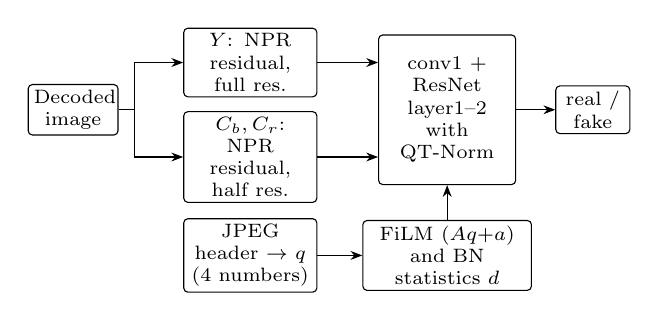
\begin{tikzpicture}[font=\scriptsize,
  box/.style={draw, rounded corners=1.5pt, align=center, inner sep=2pt, text width=#1},
  box/.default=1.55cm, arr/.style={-{Stealth[length=1.5mm]}}]
\node[box=1.0cm] (img) at (0,0) {Decoded image};
\node[box] (y) at (2.25,0.6) {$Y$: NPR residual, full res.};
\node[box] (c) at (2.25,-0.6) {$C_b,C_r$: NPR residual, half res.};
\node[box=1.6cm, minimum height=1.9cm] (net) at (4.75,0) {conv1 +\\ResNet layer1--2\\with QT-Norm};
\node[box=0.8cm] (out) at (6.6,0) {real / fake};
\node[box] (hdr) at (2.25,-1.85) {JPEG header $\rightarrow q$ (4 numbers)};
\node[box=2.0cm] (film) at (4.75,-1.85) {FiLM $(Aq{+}a)$ and BN statistics $d$};
\draw[arr] (img.east) -- ++(0.2,0) |- (y.west);
\draw[arr] (img.east) -- ++(0.2,0) |- (c.west);
\draw[arr] (y.east) -- (y.east -| net.west);
\draw[arr] (c.east) -- (c.east -| net.west);
\draw[arr] (net.east) -- (out.west);
\draw[arr] (hdr.east) -- (film.west);
\draw[arr] (film.north) -- (net.south);
\end{tikzpicture}
\caption{JA-NPR. NPR's $2{\times}2$ residual is computed on luma at full resolution and on
$2{\times}2$-averaged chroma, the resolution at which a 4:2:0 file stores colour. Every batch-norm
layer is conditioned on a four-number summary of the JPEG header.}
\label{fig:method}
\end{figure}

\subsection{Chroma-aligned NPR residual}
Let $T$ be the RGB$\rightarrow$YCbCr transform and $(Y,C)=T(x)$ with $C=(C_b,C_r)$. We compute
\begin{align}
R_Y &= Y - \up(\dn(Y)),\\
\bar C &= \mathrm{AvgPool}_{2}(C), \qquad R_C = \up\!\left(\bar C - \up(\dn(\bar C))\right),
\end{align}
where $\dn$ and $\up$ are as in Eq.~(1). The pool runs on pixels after decoding, for every file, including PNG and 4:4:4. On a 4:2:0 file the average over a cell is close to the one chroma sample that file stored, so $R_C$ compares neighbouring stored samples. Those neighbours sit on a half-resolution grid, which is a $4{\times}4$ block in the decoded image. There is no within-cell chroma left in $R_C$. On a PNG or a 4:4:4 file the same pool throws away chroma the file actually contained. As in the released NPR code, the residual is scaled by $2/3$ before conv1, which therefore sees $\tfrac{2}{3}[R_Y, R_C]/(255\,s)$. The constant $s{=}0.226$ only sets the input range. The Appendix spells out why.

The residual is linear, and the constant offsets inside $T$ cancel when you subtract a cell from itself. If chroma is residualized at full resolution instead of after the pool, the released network can be rewritten as a first convolution in YCbCr:
\begin{equation}
W'_{o,k} = s \sum_{c} W_{o,c}\, \frac{[T^{-1}]_{c,k}}{\sigma_c},
\end{equation}
where $\sigma_c$ are NPR's ImageNet channel scales. The $2/3$ factor sits on both sides and drops out. The derivation is in the Appendix. Before every training run the code checks this full-resolution identity. The largest logit gap we have recorded is $3{\times}10^{-4}$. Eq.~(3) is not that identity. Once chroma is pooled, the network at step zero is already different from the released checkpoint, and the check does not cover it. CA-NPR itself has no new weights.

\subsection{Quantization-table-conditioned normalization}
From the file header we read a descriptor
\begin{equation}
q = \big[\,\mathbb{1}_{\text{JPEG}},\ \tfrac{1}{5}\log(1+\bar Q_Y),\ \tfrac{1}{5}\log(1+\bar Q_C),\ \mathbb{1}_{4:2:0}\,\big],
\end{equation}
where $\bar Q_Y$ and $\bar Q_C$ are the mean entries of the luma and chroma tables. A PNG has $q=\mathbf{0}$. The last bit is 1 only when Pillow reports sampling code 2, which is 4:2:0. A 4:2:2 file gets the same $q$ as a 4:4:4 file with the same tables. The header cannot tell the network that 4:2:2 is subsampled. We replace each of the 24 batch-norm layers in the stem, layer1 and layer2 by
\begin{equation}
\hat h = \gamma\,\frac{h-\mu_d}{\sqrt{\sigma^2_d+\epsilon}}+\beta, \qquad
h' = \hat h \odot \big(1+g(q)\big) + b(q),
\end{equation}
with $d\in\{0,1\}$ picking one of two running-stat buffers, both copied from the released model at the start. In the code, $d$ is chosen once per batch: average $q_1$ over the batch and threshold at 0.5. That is a per-file choice in every run we report, because clean images and their JPEG copies go through in separate passes (Section~\ref{sec:train}) and each test batch is a single condition. Training uses the batch moments and updates the buffer for that $d$. Testing uses the buffer. The map $[g;b]=Aq+a$ is a linear layer per image, and $A$ and $a$ are initialized at zero, so QT-Norm does nothing to the activations on the first forward. There are 5{,}056 normalized channels, which is 50{,}560 new parameters, 1.438M to 1.488M. Parsing $q$ does not add a forward pass. The decoder has already read the header.

\subsection{Training}
\label{sec:train}
A crop of $x$ is flipped, and a JPEG copy $\tilde x$ is encoded with quality drawn uniformly from 30 to 95 and subsampling drawn from \{4:2:0, 4:4:4\}. The loss is the sum of two binary cross-entropies,
$\mathcal{L}=\mathrm{BCE}(f(x,\mathbf 0),y)+\mathrm{BCE}(f(\tilde x,q(\tilde x)),y)$,
run as two forwards so the batch-norm domain is not mixed inside a batch. Adam runs for 6 epochs at batch size 16, with learning rate $2{\times}10^{-5}$ on the pretrained weights and $10^{-3}$ on the new FiLM layers. Every trained arm uses this schedule. The fast-BN control (Section~\ref{sec:setup}) changes only the learning rate on its existing batch-norm scale and shift. We call this schedule P2.

% =====================================================================================
\section{Experimental Setup}
\label{sec:setup}
Images come from GANGen-Detection~\cite{tan2024npr}. AttGAN~\cite{he2019attgan} is $256^2$. BEGAN~\cite{berthelot2017began}, SNGAN~\cite{miyato2018sngan} and STGAN~\cite{liu2019stgan} are $128^2$. CramerGAN, InfoMaxGAN, MMDGAN, RelGAN and S3GAN appear only as unseen tests (Table~\ref{tab:data}). Each generator has 2{,}000 real and 2{,}000 fake images. For the four generators we audited, those files are PNG. AttGAN's fakes are edits of 143 source faces, so a random image split would leak faces into both sides. The split is by face: 3{,}194 train, 806 test (400 real, 406 fake), no shared face.

\begin{table}[t]
\centering
\caption{Generators used. Each has 2{,}000 real and 2{,}000 fake images.}
\label{tab:data}
\setlength{\tabcolsep}{3pt}
\footnotesize
\begin{tabular}{p{1.55cm}p{0.7cm}p{2.3cm}p{2.6cm}}
\toprule
Generator & Size & Role & Note \\
\midrule
AttGAN~\cite{he2019attgan} & $256^2$ & train and test (face split) & 143 source faces \\
SNGAN~\cite{miyato2018sngan} & $128^2$ & unseen test; trained on in held-out runs & \\
STGAN~\cite{liu2019stgan} & $128^2$ & unseen test & file statistics separate classes \\
BEGAN~\cite{berthelot2017began} & $128^2$ & unseen test & reals previously JPEG-compressed \\
CramerGAN, InfoMaxGAN, MMDGAN, RelGAN, S3GAN & -- & unseen test (held-out seed 1) & file format not audited \\
\bottomrule
\end{tabular}
\end{table}

Every model sees the PNG, JPEG 4:2:0 at Q95, 90, 70, 50 and 30, JPEG 4:4:4 at Q95 and 75, and JPEG 4:2:2 at Q85. The 4:2:2 quality is never drawn during training. Encoding is Pillow throughout this section. A different encoder would be a different experiment.

Released NPR is the authors' ProGAN checkpoint~\cite{tan2024npr}, untouched. Plain is that checkpoint fine-tuned with P2, and it is the baseline a new arm has to beat. The ablations are CA-NPR with two BN buffers and no FiLM (ycdsbn), full JA-NPR, and JA-NPR with a compression-adversarial head (CAdv). The controls are JA-NPR with FiLM's input clamped to a constant (const-$q$, same number of weights), Plain with learning rate $10^{-3}$ on the batch-norm scale and shift (fast-BN), and QT-Norm applied to the RGB residual instead of the chroma-pooled one (QT-Norm RGB).

AUC is computed on the raw logit. Balanced accuracy uses the default probability cut of 0.5, which is the same as a logit threshold of zero after the usual sigmoid. Intervals are 95\% from 1{,}000 bootstrap draws~\cite{efron1993bootstrap}. A draw resamples whole source faces when the filename identifies a face, and single images when it does not. Arm-to-arm differences use the same draws for both arms.

The pass rule was in the training script before the runs below. Against Plain, a new arm passes only if the paired interval excludes zero in its favour at Q95 and Q90 4:2:0, for both AUC and balanced accuracy, and does not exclude zero against it on PNG, on Q70, Q50 or Q30 4:2:0, or on Q95 or Q75 4:4:4.

% =====================================================================================
\section{Results}
\subsection{Main result}
Table~\ref{tab:main} and Fig.~\ref{fig:curve} are three seeds. Each seed rebuilds the face split and reshuffles the training order, so the spread is not just initialization. Released NPR stays below 0.5 at every 4:2:0 quality. The fine-tune climbs back, 0.799 at Q95 in the three-seed mean, then slides to 0.574 at Q30. JA-NPR sits above it in every JPEG column. Along 4:2:0 the gap is roughly six to thirteen points of AUC, wider at Q95 and again at Q30 than in the middle of the range. PNG is saturated for both trained models, which is why the JPEG columns are the comparison. The 4:2:2 column, Q85, was never in the training draw, and the mean still moves from 0.822 to 0.891. Section~\ref{sec:why} already noted that $q$ does not mark 4:2:2 as subsampled, so that column is not a header-detection trick.

The 0.5 threshold tells a harsher story than AUC (Table~\ref{tab:bacc}). Fine-tuned NPR is at 0.573 balanced accuracy at Q95 and 0.499 at Q30. JA-NPR is at 0.826 and 0.617 on those two columns. Fig.~\ref{fig:decomp} splits the distance from the released checkpoint into the part you get by fine-tuning on JPEG copies and the part you get by changing the model, on the same data.

\begin{figure}[t]
\centering
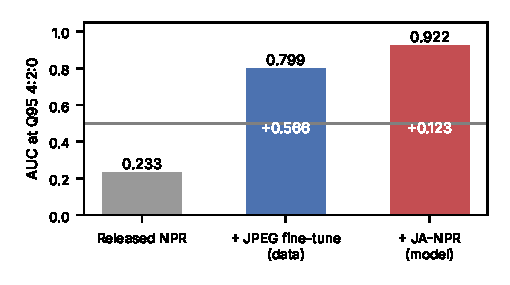
\includegraphics[width=\columnwidth]{figures/fig_decomp.pdf}
\caption{Where the improvement over the base paper comes from (AttGAN, Q95 4:2:0, mean of three
seeds). Fine-tuning on JPEG data recovers +0.566 AUC. JA-NPR adds a further +0.123 under identical
data.}
\label{fig:decomp}
\end{figure}

\begin{table*}[t]
\centering
\caption{AUC on AttGAN test faces (face-grouped split). Mean over seeds 0--2, with the min--max range in
the second line of each row. Released NPR is evaluated on seed 0 only.}
\label{tab:main}
\setlength{\tabcolsep}{4pt}
\resizebox{\textwidth}{!}{%
\begin{tabular}{lccccccccc}
\toprule
& & \multicolumn{5}{c}{JPEG 4:2:0} & \multicolumn{2}{c}{JPEG 4:4:4} & 4:2:2 \\
\cmidrule(lr){3-7}\cmidrule(lr){8-9}\cmidrule(lr){10-10}
Method (params) & PNG & Q95 & Q90 & Q70 & Q50 & Q30 & Q95 & Q75 & Q85$^\ast$ \\
\midrule
Released NPR~\cite{tan2024npr} (1.438M) & 0.956 & 0.233 & 0.245 & 0.330 & 0.323 & 0.379 & 0.876 & 0.365 & 0.317 \\
NPR + JPEG fine-tune (1.438M) & 0.999 & 0.799 & 0.810 & 0.762 & 0.676 & 0.574 & 0.989 & 0.816 & 0.822 \\
\quad {\scriptsize range over seeds} & {\scriptsize .999--1.00} & {\scriptsize .784--.818} & {\scriptsize .795--.829} & {\scriptsize .750--.773} & {\scriptsize .661--.686} & {\scriptsize .538--.602} & {\scriptsize .982--.994} & {\scriptsize .813--.820} & {\scriptsize .799--.846} \\
\textbf{JA-NPR (ours, 1.488M)} & \textbf{1.000} & \textbf{0.922} & \textbf{0.895} & \textbf{0.825} & \textbf{0.788} & \textbf{0.702} & \textbf{0.998} & \textbf{0.900} & \textbf{0.891} \\
\quad {\scriptsize range over seeds} & {\scriptsize 1.00--1.00} & {\scriptsize .889--.941} & {\scriptsize .855--.929} & {\scriptsize .782--.849} & {\scriptsize .747--.823} & {\scriptsize .699--.704} & {\scriptsize .996--1.00} & {\scriptsize .863--.919} & {\scriptsize .834--.923} \\
\bottomrule
\multicolumn{10}{l}{\scriptsize $^\ast$4:2:2 subsampling is never used in training.}
\end{tabular}}
\end{table*}

\begin{figure}[t]
\centering
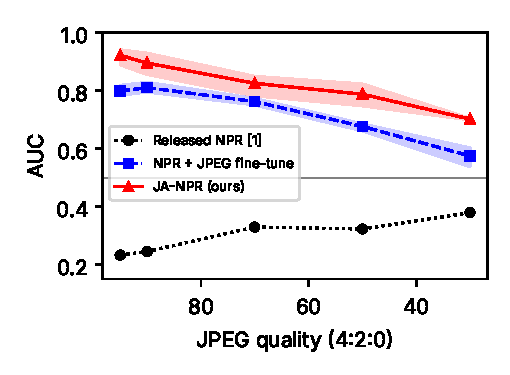
\includegraphics[width=\columnwidth]{figures/fig_quality_curve.pdf}
\caption{AUC against JPEG quality (4:2:0) on AttGAN. The lines are the mean over three seeds and
the bands show the min--max range. Values below the grey line at 0.5 are inverted.}
\label{fig:curve}
\end{figure}

\begin{table}[t]
\centering
\caption{Balanced accuracy at the default 0.5 threshold (AttGAN, mean of 3 seeds).}
\label{tab:bacc}
\setlength{\tabcolsep}{3.5pt}
\resizebox{\columnwidth}{!}{%
\begin{tabular}{lcccccc}
\toprule
Method & PNG & Q95 & Q90 & Q70 & Q50 & Q30 \\
\midrule
Released NPR & 0.802 & 0.502 & 0.501 & 0.500 & 0.500 & 0.500 \\
NPR + JPEG FT & 0.951 & 0.573 & 0.566 & 0.534 & 0.507 & 0.499 \\
\textbf{JA-NPR} & \textbf{0.998} & \textbf{0.826} & \textbf{0.804} & \textbf{0.726} & \textbf{0.685} & \textbf{0.617} \\
\bottomrule
\end{tabular}}
\end{table}

\subsection{Robustness across seeds}
Table~\ref{tab:seeds} is the paired 4:2:0 difference, seed by seed. On every seed, JA-NPR's AUC is higher than Plain's on all nine test conditions, not only the five qualities in the table. The rule we wrote down first passes on seeds 0 and 2. Seed 1 misses it: the Q90 difference is $+0.060$ with interval $[-0.001,+0.114]$, which touches zero. The point estimate is still positive. The interval does not clear the rule, and we did not edit the rule after seeing the table.

\begin{table}[t]
\centering
\caption{Paired AUC difference, JA-NPR minus NPR + JPEG fine-tune, with 95\% CI (AttGAN, 4:2:0).}
\label{tab:seeds}
\setlength{\tabcolsep}{2.5pt}
\scriptsize
\resizebox{\columnwidth}{!}{%
\begin{tabular}{lcccc}
\toprule
Cond. & Seed 0 & Seed 1 & Seed 2 \\
\midrule
Q95 & +.147 [+.094, +.201] & +.105 [+.039, +.167] & +.117 [+.066, +.165] \\
Q90 & +.122 [+.081, +.167] & +.060 [$-$.001, +.114] & +.072 [+.015, +.120] \\
Q70 & +.076 [+.025, +.127] & +.032 [$-$.027, +.094] & +.081 [+.023, +.133] \\
Q50 & +.140 [+.087, +.195] & +.062 [$-$.012, +.140] & +.131 [+.058, +.202] \\
Q30 & +.119 [+.054, +.187] & +.096 [+.013, +.183] & +.166 [+.069, +.254] \\
\midrule
Verdict & PASS & FAIL (Q90) & PASS \\
\bottomrule
\end{tabular}}
\end{table}

\subsection{Ablation and controls}
Table~\ref{tab:abl} is seed 0, one schedule, every row. ycdsbn, which is the chroma pool plus two BN buffers and no FiLM, does not beat Plain. At Q70 it is worse by 0.081, interval $[-0.150,-0.016]$, and it fails the rule. fast-BN, the same fine-tune with a higher learning rate on the existing scale and shift, picks up 0.046 at Q95. JA-NPR is ahead of fast-BN at every JPEG quality in the table, by 0.101 at Q95 with interval $[+0.051,+0.149]$. A larger step size on the old affine is not the gain.

On AttGAN the numbers inside $q$ are optional. const-$q$ has the same weights and a fixed input, and at Q95 it is within 0.002 of JA-NPR, interval $[-0.021,+0.025]$. What this generator is using is a JPEG path through the normalization: a second buffer, selected by the JPEG flag, and a learned per-channel scale and shift. We did not get that from either piece in isolation. ycdsbn has the second buffer and failed. fast-BN has a faster affine and no second buffer, and it moved the Q95 number only a little.

QT-Norm on the RGB residual also passes the rule, and at Q70, Q50 and Q30 it is the highest row in Table~\ref{tab:abl}. Against that RGB version, adding the chroma pool changes Q95 4:2:0 by $+0.034$ $[+0.001,+0.066]$ and Q75 4:4:4 by $-0.028$ $[-0.052,-0.010]$. The pool is not the main AttGAN effect, and the sign depends on the test. The compression-adversarial head~\cite{ganin2015dann}, the same idea as in~\cite{tao2025oddn,li2025plada}, adds 0.002 at Q95. The adversary's accuracy fell to 0.53 in epoch 4 and was back at 0.998 at the end, so the trunk did not stay invariant to compression. Fig.~\ref{fig:abl} is the same comparison as a plot.

\begin{figure}[t]
\centering
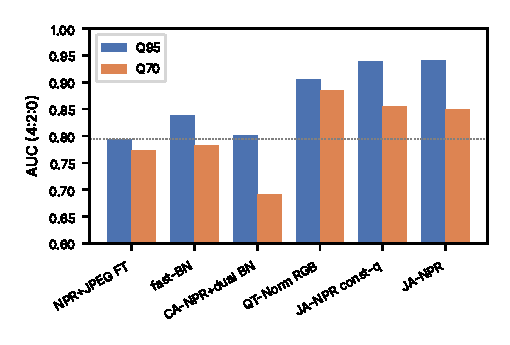
\includegraphics[width=\columnwidth]{figures/fig_ablation.pdf}
\caption{Ablation and controls (AttGAN, seed 0). The dotted line is the fine-tuned NPR at Q95.
Only variants that combine separate clean/JPEG statistics with learnable modulation clearly beat
it at both qualities.}
\label{fig:abl}
\end{figure}

\begin{table}[t]
\centering
\caption{Ablation and controls on AttGAN (seed 0, AUC, 4:2:0). All rows: same data and protocol.
Rows come from three runs of the same seed; arms repeated across runs differ by at most 0.006.}
\label{tab:abl}
\setlength{\tabcolsep}{3pt}
\resizebox{\columnwidth}{!}{%
\begin{tabular}{lcccccc}
\toprule
Variant & Q95 & Q90 & Q70 & Q50 & Q30 & Params \\
\midrule
NPR + JPEG fine-tune (Plain) & 0.794 & 0.807 & 0.773 & 0.683 & 0.583 & 1.438M \\
Plain, fast-BN (control) & 0.839 & 0.839 & 0.783 & 0.711 & 0.612 & 1.438M \\
CA-NPR + dual BN (ycdsbn) & 0.801 & 0.794 & 0.692 & 0.638 & 0.551 & 1.438M \\
QT-Norm on RGB residual & 0.906 & 0.908 & \textbf{0.885} & \textbf{0.839} & \textbf{0.728} & 1.488M \\
JA-NPR, const-$q$ (control) & 0.938 & 0.913 & 0.855 & 0.811 & 0.693 & 1.488M \\
\textbf{JA-NPR} & 0.940 & \textbf{0.929} & 0.849 & 0.823 & 0.702 & 1.488M \\
JA-NPR + CAdv & \textbf{0.943} & 0.929 & 0.850 & 0.820 & 0.703 & 1.488M$^\dagger$ \\
\bottomrule
\multicolumn{7}{l}{\scriptsize $^\dagger$ plus 513 training-only parameters.}
\end{tabular}}
\end{table}

\subsection{Generators never seen in training}
Training on AttGAN and SNGAN, with 128-pixel crops, and testing the full 4{,}000 images of STGAN and BEGAN gives Table~\ref{tab:held} and Fig.~\ref{fig:held}. On STGAN the fine-tune sits at or below 0.5 for every JPEG column. JA-NPR passes the rule there. The Q95 paired gain is $+0.248$ $[+0.219,+0.280]$, and at Q30 it is still $+0.159$. BEGAN also passes the rule on the differences, but the absolute AUC at Q95 and Q90 stays under one half. Those real images were JPEG-compressed before anyone assembled the dataset. Section~\ref{sec:shortcut} is that check. Trained on AttGAN only, seed 0, the same Q95 comparison is 0.417 to 0.760 on BEGAN and 0.344 to 0.582 on STGAN, and 0.474 to 0.501 on SNGAN, which is no real movement.

\begin{table}[t]
\centering
\caption{Held-out generators (trained on AttGAN+SNGAN, seed 0, AUC).}
\label{tab:held}
\setlength{\tabcolsep}{2.6pt}
\resizebox{\columnwidth}{!}{%
\begin{tabular}{llcccccc}
\toprule
Test & Method & PNG & Q95 & Q90 & Q70 & Q50 & Q30 \\
\midrule
\multirow{2}{*}{STGAN} & NPR + JPEG FT & 0.999 & 0.515 & 0.478 & 0.466 & 0.447 & 0.431 \\
 & \textbf{JA-NPR} & \textbf{1.000} & \textbf{0.764} & \textbf{0.695} & \textbf{0.617} & \textbf{0.586} & \textbf{0.590} \\
\midrule
\multirow{2}{*}{BEGAN} & NPR + JPEG FT & 0.982 & 0.240 & 0.153 & 0.240 & 0.262 & 0.288 \\
 & JA-NPR & 1.000 & 0.483 & 0.449 & 0.591 & 0.730 & 0.764 \\
\bottomrule
\end{tabular}}
\end{table}

\begin{figure}[t]
\centering
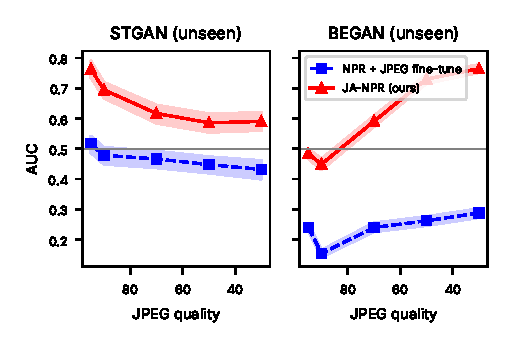
\includegraphics[width=\columnwidth]{figures/fig_heldout.pdf}
\caption{Unseen generators (trained on AttGAN+SNGAN). The bands are 95\% bootstrap CIs.}
\label{fig:held}
\end{figure}

\subsection{What the quantization table adds on unseen generators}
The held-out run with the controls included (Table~\ref{tab:ctrl}) is where the header values show up. On STGAN, JA-NPR beats const-$q$ by 0.117 at Q95, interval $[+0.103,+0.132]$, then by 0.102, 0.065 and 0.041 at Q90, Q70 and Q50, and by 0.109 on the 4:2:2 files it was not trained on. With two generators in training, the same comparison on the seen AttGAN faces is $+0.058$ at Q95, interval $[+0.026,+0.094]$. That is a different training mixture from the AttGAN-only ablation, where const-$q$ matched JA-NPR. fast-BN fails the rule on both unseen generators in this table.

\begin{table}[t]
\centering
\caption{Controls in the held-out setting (trained on AttGAN+SNGAN, seed 0, AUC on unseen STGAN,
4:2:0).}
\label{tab:ctrl}
\setlength{\tabcolsep}{3pt}
\resizebox{\columnwidth}{!}{%
\begin{tabular}{lccccc}
\toprule
Variant & Q95 & Q90 & Q70 & Q50 & Q30 \\
\midrule
NPR + JPEG fine-tune & 0.515 & 0.478 & 0.466 & 0.448 & 0.431 \\
Plain, fast-BN (control) & 0.546 & 0.520 & 0.501 & 0.457 & 0.435 \\
JA-NPR, const-$q$ (control) & 0.645 & 0.592 & 0.551 & 0.544 & 0.564 \\
\textbf{JA-NPR (reads header)} & \textbf{0.762} & \textbf{0.694} & \textbf{0.616} & \textbf{0.586} & \textbf{0.589} \\
\bottomrule
\end{tabular}}
\end{table}

A second seed, same AttGAN+SNGAN training, is scored on seven unseen generators: STGAN, BEGAN, and CramerGAN, InfoMaxGAN, MMDGAN, RelGAN, S3GAN, each with 4{,}000 images (Table~\ref{tab:seven}). STGAN repeats. JA-NPR is 0.159 above const-$q$ at Q95, interval $[+0.140,+0.181]$, and 0.282 above the fine-tune ($0.519$ to $0.802$).

The header effect does not have one sign. It is clearly positive on STGAN. On BEGAN it is positive at Q95 only; const-$q$ is better from Q90 down to Q30. CramerGAN, MMDGAN and RelGAN move by about nothing once you look at the intervals, aside from a small positive CramerGAN interval that still fails the full rule for JA-NPR. InfoMaxGAN and S3GAN go the other way, $-0.117$ and $-0.053$, and both intervals exclude zero.

The normalization, constant input included, travels further than the table values. Against the fine-tune it passes the rule on four of the seven generators with JA-NPR and on five with const-$q$. The largest Q95 jump is RelGAN, 0.397 to 0.762. InfoMaxGAN goes from 0.629 down to 0.520. S3GAN is weak before any JPEG is applied: the fine-tune reaches only 0.650 on the PNGs. Fig.~\ref{fig:seven} puts the Q95 bars next to each other.

\begin{figure}[t]
\centering
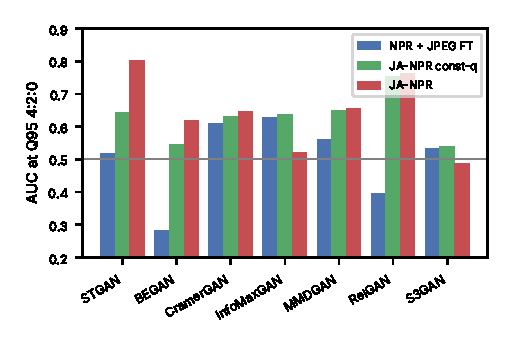
\includegraphics[width=\columnwidth]{figures/fig_seven.pdf}
\caption{AUC at Q95 4:2:0 on seven unseen generators (trained on AttGAN+SNGAN, seed 1). The grey
line marks chance.}
\label{fig:seven}
\end{figure}

\begin{table}[t]
\centering
\caption{Seven unseen generators (trained on AttGAN+SNGAN, seed 1). AUC at Q95 4:2:0, the
pre-registered verdict against the fine-tuned NPR (P = pass, F = fail), and the paired effect of
reading the header (JA-NPR minus const-$q$, 95\% CI).}
\label{tab:seven}
\setlength{\tabcolsep}{2.5pt}
\resizebox{\columnwidth}{!}{%
\begin{tabular}{lccccc}
\toprule
Unseen & NPR + & const-$q$ & JA-NPR & Verdict & Header effect \\
generator & JPEG FT & & & ($q$/JA) & at Q95 \\
\midrule
STGAN & 0.519 & 0.642 & \textbf{0.802} & P / P & +0.159 [+0.140, +0.181] \\
BEGAN$^\ast$ & 0.281 & 0.546 & 0.619 & P / P & +0.073 [+0.054, +0.090] \\
CramerGAN & 0.609 & 0.631 & 0.647 & P / F & +0.016 [+0.004, +0.029] \\
InfoMaxGAN & 0.629 & 0.637 & 0.520 & F / F & $-$0.117 [$-$0.133, $-$0.104] \\
MMDGAN & 0.560 & 0.648 & 0.654 & P / P & +0.006 [$-$0.007, +0.019] \\
RelGAN & 0.397 & 0.753 & 0.762 & P / P & +0.009 [$-$0.003, +0.023] \\
S3GAN & 0.532 & 0.540 & 0.487 & F / F & $-$0.053 [$-$0.071, $-$0.037] \\
\bottomrule
\multicolumn{6}{l}{\scriptsize $^\ast$const-$q$ is better than JA-NPR at Q90--Q30 on BEGAN.}
\end{tabular}}
\end{table}

We do not have a test of the following, so it stays a guess. FiLM sees AttGAN and SNGAN and learns how those generators' features move when the header changes. STGAN is also a face editor, and a correction fit on AttGAN may land in the right place. InfoMaxGAN and S3GAN need not move the same way under the same table, and then the same correction is applied to a different residual. const-$q$ cannot make a quality-specific correction, which fits it helping less on STGAN and hurting less on the generators where JA-NPR goes down. Training on a wider set of generators, or shrinking the FiLM weights, would be the experiment. We have not run it.

\subsection{Prior compression as a shortcut}
\label{sec:shortcut}
BEGAN reals were already JPEG images when the dataset was built. To see whether that is why high-quality JPEG AUC stays low, we compressed the fake images once at Q90, saved them as PNG, and left the reals alone. Re-encoding both classes again barely moves the score. JA-NPR trained on AttGAN scores 0.760 on the original BEGAN JPEGs at Q95 and 0.711 on this control. Prior compression of the reals does not explain the JPEG column.

It does explain the PNG column of the control. On those uncompressed files, every model we tried ranks the pre-compressed fakes as more real than the reals. AUC falls from about 1 to 0.267 for Plain, 0.389 for JA-NPR, and 0.015 for QT-Norm RGB. The training has picked up ``old JPEG traces mean real.'' Plain has the same habit. It is the data and the protocol, not a quirk of FiLM.

\subsection{How the method evolved}
The order of experiments is worth writing down, because the explanation changed after the controls.

The released model at Q95 is inverted on 4:2:0 and not on 4:4:4, and the colour probe in Section~\ref{sec:why} says the decoder's chroma is part of the reason. Fine-tuning on JPEG copies, under the earlier P1 schedule, lifts Q95 from 0.233 to 0.829 and still leaves the 0.5 threshold near chance. That fine-tune is the baseline. A projection onto quantization-consistent $2{\times}2$ cells, a feature-consistency loss, and test-time AdaBN did not beat it (Table~\ref{tab:fail}). Under P1 the chroma-aligned residual improved ranking by 0.076 at Q95, and separate BN statistics improved balanced accuracy from 0.549 to 0.750. Together they were $+0.090$ at Q95 and $-0.109$ at Q70. FiLM from the header, trained on qualities from 30 to 95, is what removed that trade-off. The rule then passes on two of the three P2 seeds (Tables~\ref{tab:main} and~\ref{tab:seeds}).

The AttGAN controls changed what we were willing to say. const-$q$ matches JA-NPR. fast-BN does not. On this generator the gain is the JPEG path in the normalization, not the particular table means (Table~\ref{tab:abl}). The header claim only comes back on unseen generators, and only on some of them: STGAN on two seeds, mixed signs on the other six (Table~\ref{tab:seven}).

\subsection{Alternatives that failed}
\label{sec:fail}
Table~\ref{tab:fail} is the rest of what we tried before settling on JA-NPR. P1 is the earlier schedule, JPEG qualities 75 to 95 and 4:2:0 only. P2 is Section~\ref{sec:train}. Under P1 the fine-tune is at 0.829 at Q95, so the deltas below are against that number, not against Table~\ref{tab:main}. QC-NPR forces the decoded image onto $2{\times}2$-constant images that sit inside the quantization bins, and it strips more signal than it repairs. The consistency loss left the predictions where they were. Test-time AdaBN~\cite{li2018adabn} on the released weights moved a 600-image Q95 4:2:0 audit from 0.289 to 0.258, the wrong direction. The P1 trade-off, $+0.090$ at Q95 and $-0.109$ at Q70 for CA-NPR with dual BN, is why the FiLM layer was added. Under P2 that same arm still fails, now by 0.081 at Q70.

\begin{table}[t]
\centering
\caption{Failed or partial alternatives (AttGAN, seed 0, AUC at Q95 4:2:0 unless noted).}
\label{tab:fail}
\setlength{\tabcolsep}{2pt}
\scriptsize
\resizebox{\columnwidth}{!}{%
\begin{tabular}{p{3.3cm}p{4.9cm}}
\toprule
Alternative & Outcome \\
\midrule
QC-NPR front-end (P1) & 0.693 vs.\ 0.829 ($-$0.136 [$-$0.196, $-$0.080]); worse \\
Feature consistency loss (P1) & identical to baseline (0.829) \\
Test-time AdaBN, released model & 0.289$\to$0.258 at Q95 4:2:0 (600-image audit) \\
Dual BN stats only (P1) & AUC +0.014 (n.s.); balanced acc.\ 0.549$\to$0.750 \\
CA-NPR + dual BN (P1) & +0.090 at Q95, but $-$0.109 at Q70 \\
CA-NPR + dual BN (P2, Table~\ref{tab:abl}) & fails rule ($-$0.081 at Q70) \\
Compression-adversarial head & +0.002 (n.s.); adversary acc.\ 0.998 at end \\
Block-position input & no added signal: $8{\times}8$ blocks never split $2{\times}2$ cells \\
\bottomrule
\end{tabular}}
\end{table}

\subsection{Can the header reveal the label?}
QT-Norm reads the header, so we checked that the header is not a label in disguise. The 16{,}000 original images of AttGAN, BEGAN, SNGAN and STGAN are PNG, real and fake, so $q=\mathbf{0}$ for both classes. Every JPEG test re-encodes both classes with the same settings, so they receive the same $q$. The network can see how the file was compressed. It cannot see the class in $q$. We did not audit the file format of the five extra generators. Their JPEG rows are still matched across classes. Their PNG rows are not something we can vouch for.

% =====================================================================================
\section{Limitations}
\label{sec:limits}
Nine generators, 4{,}000 images each, and training on AttGAN, or on AttGAN plus SNGAN in the held-out runs. The single-generator result is three seeds, and one of them misses the rule on Q90. The held-out header comparison is two seeds, the second of which covers the seven unseen sets. The AttGAN-only controls are one seed. That is enough to see the pattern and not enough to treat the seed-1 miss as noise we can ignore.

A 300-image audit finds an $8{\times}8$ JPEG grid in BEGAN reals and not in BEGAN fakes ($z{=}{+}8.6$ on a block-boundary statistic). File size and related metadata separate STGAN classes at AUC 0.954 and BEGAN at 0.829, without looking at pixels. On AttGAN, the set the main table uses, the same metadata probe is 0.578, and the block statistic points the other way, fakes higher, $z{=}{-}4.3$. JA-NPR and Plain see the same pixels and, when both are trained, the same images. The gaps between them are relative. Absolute STGAN and BEGAN AUCs should be read next to those audits.

SNGAN stays near 0.5 under JPEG even when it is in the training set. For that generator the NPR trace does not seem to survive compression in a form either model can rank. Calibration is a separate failure. In the held-out AttGAN run at Q50, AUC is 0.720 and only 11\% of real images are accepted at the 0.5 cut.

When the training set is AttGAN alone, swapping the header vector for a constant does not change the AttGAN number. With AttGAN and SNGAN both in training, the same swap costs 0.058 on AttGAN and a large, repeated amount on STGAN, and it costs the wrong sign on InfoMaxGAN and S3GAN. We have not measured whether the residual itself is less sensitive to subsampling after training. The AUC can move because later layers compensate for an input effect that is still there. The chroma pool's own share, against RGB QT-Norm, is small and changes sign with the test condition.

InfoMaxGAN and S3GAN fail the rule for the normalization as well as for the header. JA-NPR is not a cross-generator JPEG detector. Section~\ref{sec:shortcut} is the prior-compression shortcut, and it is shared. We only used Pillow, and only one encode. If a file is compressed twice, $q$ describes the last table.

% =====================================================================================
\section{Conclusion}
The released NPR checkpoint does not fade evenly under JPEG. At quality 95 the AttGAN ranking survives 4:4:4 and inverts under 4:2:0, which is what you would expect if the detector were reading colour differences the decoder had filled in. JA-NPR keeps the $2{\times}2$ residual. It computes the chroma part after a $2{\times}2$ average of the decoded pixels, and it gives batch-norm a clean buffer, a JPEG buffer, and a FiLM layer on a four-number header. That is 0.05M parameters on top of the NPR trunk.

On AttGAN, with a fine-tune that saw the same images, the JPEG columns all move in JA-NPR's favour, including qualities and a 4:2:2 test that the pass rule was not written around. The constant-input control says the AttGAN movement is the normalization path, not the table entries and not the learning rate. The chroma pool is a smaller, signed difference once QT-Norm is already on the RGB residual. Held-out generators split the story. The normalization passes our rule on four of seven, five if the header is clamped, with RelGAN the large positive case and InfoMaxGAN a clear loss. The table values themselves help STGAN on both seeds and hurt two other generators.

What is still open is narrower than ``robust detection.'' We do not know when a header-conditioned FiLM transfers, the seed count is small, the prior-compression shortcut is still in every trained arm, and we have not tried a second encode or a second compressor. Low-quality AUC and the 0.5 threshold are already different measurements on the held-out AttGAN run.

\section*{Code and Data Availability}
Code, run logs, result CSVs and trained weights: \url{https://github.com/pvkacode/JA-NPR}.

\appendix
\section*{Appendix: Exactness of the first-layer re-expression}
NPR normalizes each RGB channel as $x^n_c=(x_c/255-\mu_c)/\sigma_c$, and its residual is
$R^{rgb}_c=x^n_c-\mathcal{U}(\mathcal{D}(x^n_c))$. The operator $\mathcal{U}\mathcal{D}$ is linear
and maps constants to themselves, so $\mu_c$ cancels and $R^{rgb}_c=(x_c-\mathcal{U}\mathcal{D}x_c)
/(255\,\sigma_c)$. JPEG's colour transform is affine, $y=Tx+o$, so $x=T^{-1}(y-o)$. The offset $o$
cancels in the residual in the same way, giving
\begin{equation}
R^{rgb}_c=\frac{1}{255\,\sigma_c}\sum_k [T^{-1}]_{c,k}\,R^{ycc}_k,\qquad
R^{ycc}_k=y_k-\mathcal{U}\mathcal{D}y_k .
\end{equation}
A convolution with weights $W_{o,c}$ is linear in its input channels, so
\begin{equation}
\sum_c W_{o,c}*R^{rgb}_c=\sum_k W'_{o,k}*\frac{R^{ycc}_k}{255\,s},\qquad
W'_{o,k}=s\sum_c W_{o,c}\frac{[T^{-1}]_{c,k}}{\sigma_c},
\end{equation}
which is Eq.~(4). The identity holds for any spatial kernel, stride and zero padding, and the scale
$s$ cancels, so it only sets the numerical range of the input. We checked it with random images
and filters independently of our training code. The two sides agree to a relative error of about
$5{\times}10^{-7}$, which matches the 6-digit rounding of the standard's colour coefficients
($\|T^{-1}T-I\|_{\max}\approx 6{\times}10^{-7}$). The common factor $2/3$ that NPR applies before conv1
multiplies both sides and is omitted. CA-NPR then changes only one thing: the chroma residual is
computed at half resolution (Eq.~(3)) instead of at full resolution. Neither the identity nor our
numerical check of it covers that pooled path.

\bibliographystyle{IEEEtran}
\bibliography{refs}

\end{document}
